\newcommand{\sheetnum}{%
	01
}
%\setcounter{section}{\sheetnum-3}
\newcommand{\tutorialtitle}{%
    Introduction and the Connectionist Neuron
}
\newcommand{\tutorialtitleshort}{%
	Intro \& Perceptron
}
% for slides
\subtitle{\sheetnum \tutorialtitle}

% The following use of algroithms does not work well with the notes:
%
%
%
%
% instead use the following for your algorithms:
%
%\begin{figure}[!t]
%\removelatexerror
%\begin{algorithm}[H]
    % your aglo here
    %\label{alg:algolabel}
    %\caption{algocaption}
%\end{algorithm}
%\end{figure}
%\begin{algorithm}
% Below is the definition for the command \removelatexerror:
\makeatletter
\newcommand{\removelatexerror}{\let\@latex@error\@gobble}
\makeatother{}

\DeclarePairedDelimiter\set\{\}

\begin{document} %%%%%%%%%%%%%%%%%%%%%%%%%%%%%%%%%%%%%%%%%%%%%%%%%%%%%%%

\sheet{\sheetnum}{\tutorialtitleshort}

\ttopic{\tutorialtitle}

\columnratio{0.2,0.8}\textbf{}
\begin{paracol}{2}
%\setlength{\columnseprule}{0.1pt}
%\setlength{\columnsep}{5em}

\begin{rightcolumn}

% notes version will ignore it
\begin{frame}
\titlepage
\end{frame}

\begin{frame}
\tableofcontents
\end{frame}

\mode<all>
\section{Learning Paradigms}

\begin{frame}\frametitle{\secname}

\mode<article>{
There are three learning paradigms in machine learning:
}
\begin{itemize}
\item Supervised learning\notesonly{. Learning with a teacher (cf. \sectionref{sec:supervised}).}
\item Unsupervised learning\notesonly{. Learning only from observations, without a teacher (cf. \sectionref{sec:unsupervised}).}
\item Reinforcement learning\notesonly{. This is about maximizing reward (cf. \sectionref{sec:reinforcement}).}
\end{itemize}
\mode<article>{
It is possible to understand the differences between them by describing
\begin{inparaenum}[(i)]
    \item the data each of them deals with and
    \item the objective that each is trying to model
\end{inparaenum}
}
\mode<presentation>{

Differences: Data \& objective model.
}

\end{frame}


\subsection{Supervised learning} \label{sec:supervised}

\begin{frame}\frametitle{\subsecname}

\mode<article>Supervised learning is\mode<all>essentially function fitting.

\underline{Data}:\\
\mode<presentation>{\vspace{5mm}}

Consider this dataset of tuples:
\begin{equation}
\label{eq:tuples}
\left( \vec x^{(1)}, \vec y_T^{(1)} \right) \,,\, \ldots \,,\, \left( \vec x^{(\alpha)}, \vec y_T^{(\alpha)} \right) \,,\, \ldots \,,\, \left( \vec x^{(p)}, \vec y_T^{(p)} \right)
\end{equation}

\mode<article>{
where,
\begin{itemize}
\item[] $\vec x$ denotes the observation with $N$ components. $\vec x = (x_1, x_2, \ldots x_N)$, $\vec x \in \R^N$ (e.g. pixel values in an image)
\item[] $\vec y_T$ denotes the label assigned to this observation. It is also referred to as the ground truth.
When $y_T \in \R$ or $\vec y_T \in \R^M$, we are looking at a regression problem (e.g. predicting house prices, object localization - bounding box regression (x, y, w, h)).\\
When $y_T \in \{ 0, 1\}$, we refer to this as a binary classification problem (e.g. is this a cat or a dog).\\
When $y_T \in \{ 0, \ldots, K-1\}$, we refer to this as a multi-class classification problem (e.g. which letter is this?).
\item[] $p$ denotes the size of the dataset (i.e. how many labeled observations we have.)
\item[] The superscript $^{(\alpha)}$ denotes the index of a particular sample within the dataset. $\alpha = 1 , \ldots, p$
\item[] The samples are often assumed to be \emph{independent and identically distributed} (\iid).
\end{itemize}
}

%\end{frame}
\pause
%\begin{frame}

\underline{Objective model}:\\
\mode<presentation>{\vspace{5mm}}
\notesonly{Supervised learning algorithms are used to }find a function that maps observations to their label(s)\notesonly{ which represents some concept or value.
This mapping can be described in the form of:}
\begin{itemize}
\item a discrimination function $\vec y = \vec f(\vec x)$, \\ 

\notesonly{
where $\vec f(\cdot)$ denotes a vector valued function }$\vec f: \R^N \rightarrow \R^M$
\item a conditional distribution $P(\,\vec y \,|\, \vec x\,)$.
\end{itemize}

\end{frame}

\subsection{Unsupervised learning} \label{sec:unsupervised}

\begin{frame}\frametitle{\subsecname}

\mode<article>
Unsupervised learning tries to find 
\mode<all>
 interesting directions and/or structure in the data using only observations $\vec x \in \R^N$.

\underline{Data}:

A dataset of observations:
\begin{equation}
\label{eq:observations}
%\vec x^{(1)} \,,\, \ldots \,,\, \vec x^{(\alpha)} \,,\, \ldots \,,\, \vec x^{(p)}
\vec X = 
\left(
\begin{array}{cccccc}
\Big| & \Big| & & \Big| & & \Big| \\[3mm]
\vec x^{(1)} & \vec x^{(2)} & \cdots & \vec x^{(\alpha)} & \cdots & \vec x^{(p)}\\[2mm]
\Big| & \Big| & & \Big| & & \Big|
\end{array}
\right) \in \R^{N \times p}
\end{equation}
\notesonly{
where $p$ denotes the number of observations (i.e. size of the dataset) and $N$ denotes the number of dimensions.}
\slidesonly{
where 
\begin{itemize}
\item[] $p$ \corresponds\, no. of observations (often \iid)
\item[] $N$ \corresponds\, no. of dimensions
\end{itemize}
}
\notesonly{
The samples are often assumed to be \iid, but algorithms for handling sequential data also exist.

Example: $\vec x$ could represent user ratings, pixel values in images.
}
\end{frame}
\begin{frame}

\underline{Objective model}:
\mode<presentation>{\vspace{5mm}}
\mode<article>{
An unsupervised learning algorithm is used to capture structure or directions in the data. This can be achieved by finding:
}
\begin{itemize}
\item the underlying distribution $P(\vec x)$ that generated this data (e.g. density estimation),
\item $\vec z := \vec f(\vec x)$, where $\vec z$ is a measure of 
\begin{itemize}
\item possible structure such as clustering or grouping in the data ($\vec z \in {0,\ldots,K-1}$), \\

and/or

\item possible directions in the data, by finding another continuous space for describing this data. \\

Example: dimensionality reduction, $\vec z \in \R^M$ with $M < N$.

\end{itemize}
\end{itemize}

\end{frame}

\newpage

\subsection{Reinforcement learning} \label{sec:reinforcement}

\begin{frame}\frametitle{\subsecname}

Reinforcement learning is a about what actions to take in which situations in order to maximize some reward.
This implies that learning happens through an interaction of the agent with its environment.

\end{frame}

\begin{frame}

\underline{Data}:

Our data consists of a sequence. Each time step is described by 

\begin{itemize}
\item a state $\vec x \in \mathcal{X}$ or $\vec x \in \R^N$, e.g. $\mathcal{X} := \{ \vec x_1, \ldots, \vec x_S\} \subset \{0,1\}^S$ (1-out-$S$ encoding)
\pause
\item an action $\vec a$ which can be taken by the agent:\\

$\vec a \in \mathcal{A}$ or $\vec a \in \R^M$, e.g. $\mathcal{A} := \{ \vec a_1, \ldots, \vec a_A\} \subset \{0,1\}^A$ (1-out-$A$ encoding)
\pause
\item a reward $r \in \R$ or $r \in \{0,1\}$, e.g. $r \in \{\text{``cheese''},\text{``no cheese''}\}$.

\end{itemize}
\pause
\mode<article>{Each time step describes what reward was received when performing some action while in some state. 
The sequence we observe becomes:}

\begin{align}
\label{eq:chain}
\left\{\vec x^{(t)}, \vec a^{(t)}, r^{(t)}\right\}_{t=0}^{p} = 
\left( \vec x^{(0)}, \vec a^{(0)}, r^{(0)} \right) \,,\, \ldots \,,\, \left(\vec x^{(p)}, \vec a^{(p)}, r^{(p)} \right)
\end{align}

\question{Can we still assume \iid?}

\mode<article>{
-Since we observe sequential data, we no longer assume \iid \emph{within} a sequence. But if we have multiple sequences, we can assume \iid \emph{across} sequences.
}

\end{frame}

\begin{frame}

Example:
\begin{itemize}
\item $\vec x \; \corresponds$ position in a maze
\item $\vec a \; \corresponds$ movement direction (velocity), e.g. turn left/right
\item $r \; \corresponds$ found the cheese, found smaller piece of cheese. A negative reward, ``punishment'' is also possible.
\end{itemize}
\end{frame}


\begin{frame}
    \mode<presentation>{
    \begin{figure}[h]
        \centering
        \only<1>{
        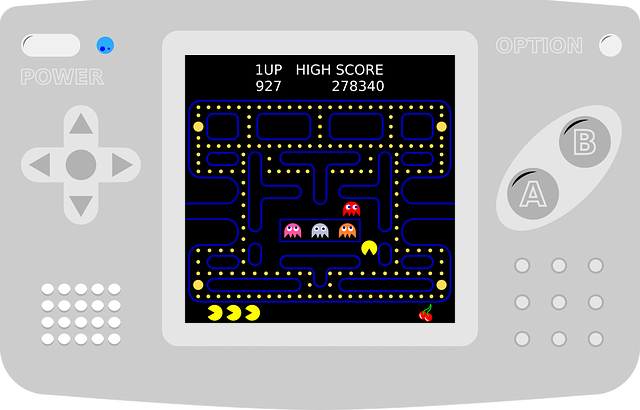
\includegraphics[height=5cm]{img/handheld-game-console-2134571_640}
        }
        \only<2>{
        
\includegraphics[height=3cm]{img/babyrajeshraj-1087832_640}
        }
    \end{figure}
    }
    
\question{What would be a state/action/reward here?}

\end{frame}

\mode<article>{
\begin{figure}[ht]
     \centering
     \savebox{\imagebox}{
	 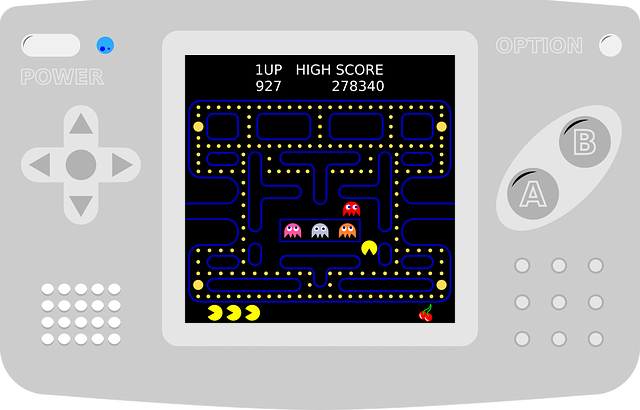
\includegraphics[width=0.2\textwidth]{img/handheld-game-console-2134571_640}}%
     \begin{subfigure}[t]{0.35\textwidth}
         \centering
         \usebox{\imagebox}% Place largest image
     \end{subfigure}
     \hspace{1mm}
     \begin{subfigure}[t]{0.25\textwidth}
         \centering
         \raisebox{\dimexpr.5\ht\imagebox-.5\height}{% Raise smaller image into place
         
\includegraphics[width=0.5\textwidth]{img/babyrajeshraj-1087832_640}
         }
     \end{subfigure}
     \caption{Representing games for reinforcement learning}
\end{figure}
}

\begin{frame}

\underline{Objective model}:\\
\mode<presentation>{\vspace{5mm}}
Reinforcement learning can be used to:
\begin{itemize}
\item select the optimal action when arriving at a state: $\vec a^* = \vec f(\vec x, r)$
\item find the transition model $P(\vec x^{(t)}\,|\,\vec x{(t-1)}, \vec a^{(t-1)})$, where $t$ is a time step within the sequence.
\end{itemize}
\pause
\question{Would you regard reinforcement learning as supervised or unsupervised learning?}

\end{frame}

\newpage

\subsection{Summarized overview}

\begin{frame}

\begin{table}[!h]

\makebox[1 \textwidth][c]{       %centering table
\resizebox{0.85 \textwidth}{!}{   %resize table
\label{tab:summary} 
\begin{tabular}{l||l|l}
                       & \multicolumn{1}{c|}{Data}                                                   & \multicolumn{1}{c}{Objective model}                                                                                                 \\ \hline \hline
\begin{tabular}[c]{@{}l@{}}Supervised\\ learning\end{tabular}    & \begin{tabular}[c]{@{}l@{}}\multicolumn{1}{c}{$\left( \vec x^{(1)}, \vec y_T^{(1)} \right) \,,\, \ldots  \,,\, \left( \vec x^{(p)}, \vec y_T^{(p)} \right)$}
\\[2mm] \qquad\qquad \rotatebox[origin=c]{180}{$\Lsh$} label $\R$, $\R^M$,$\{0,1\}$,\\ \qquad\qquad\qquad$\{0,\ldots,K-1\}$\\[2mm] \,\quad\, \rotatebox[origin=c]{180}{$\Lsh$} observation $\R^N$, often iid.\end{tabular} & \begin{tabular}[c]{@{}l@{}}\\[1mm]discrimination function\\ $\vec y = \vec f(\vec x)$\\ \\ conditional distribution\\ $P(\vec y | \vec x)$\\[1mm]\end{tabular}                                                   \\ \hline
\begin{tabular}[c]{@{}l@{}}Unsupervised\\ learning\end{tabular}   & \begin{tabular}[c]{@{}l@{}}\multicolumn{1}{c}{$\vec x^{(1)},\ldots,\vec x^{(p)} \in \R^N$}\\[2mm] observations often iid.\end{tabular}         & \begin{tabular}[c]{@{}l@{}}\\generative model/\\ data distribution $P(\vec x)$ \\[2mm] clustering: \\ $f(\vec x): \R^N \mapsto \{0,\ldots,K-1\}$\\[2mm] dimensionality reduction: \\ $\vec f(\vec x): \R^N \mapsto \R^M $\\[2mm]\end{tabular} \\ \hline
\begin{tabular}[c]{@{}l@{}}Reinforcement\\ learning\end{tabular}  & \begin{tabular}[c]{@{}l@{}} \\ \multicolumn{1}{c}{$\left( \vec x^{(0)}, \vec a^{(0)}, r^{(0)} \right) \,,\, \ldots \,,\, \left(\vec x^{(p)}, \vec a^{(p)}, r^{(p)} \right)$}\\[2mm] \;\qquad\qquad\quad \rotatebox[origin=c]{180}{$\Lsh$} reward $r \in \R$\\ \;\qquad\quad \rotatebox[origin=c]{180}{$\Lsh$} action $\vec a \in \R^M$ or $\{0,1\}^A$\\ \;\quad \rotatebox[origin=c]{180}{$\Lsh$} state $\vec x \in \R^N$ or $\{0,1\}^S$\\[2mm] \end{tabular}   & \begin{tabular}[c]{@{}l@{}}select optimal action:\\ $\vec a^* = \vec f(\vec x,r)$\\[1mm] transition model:\\ $P(\vec x^{(t)}\,|\,\vec x{(t-1)}, \vec a^{(t-1)})$\end{tabular}                                                          
\\ \hline
\end{tabular}
} %close resize
} %close centering
%\caption{Summary of learning paradigms} % makes table shift in a strange way
\end{table}

\end{frame}



\mode*

\newpage

\mode<all>
\section{Connectionist Neuron (Perceptron)}

\begin{frame}\frametitle{\secname}

A neuron is a computational unit for processing information. 

\question{What does a connectionist neuron compute?}\\

\pause
- A connectionist neuron is a type of neuron model which measures for a feature within an observation (a data point). It is a feature detector/extractor e.g. edge detector, above or below a threshold.

\end{frame}

\begin{frame}
A connectionist neuron's response to 1D data:

\begin{figure}[ht]
     \centering
     \savebox{\imagebox}{
	 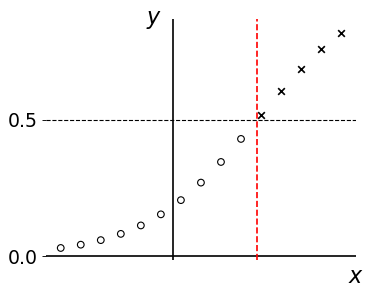
\includegraphics[width=0.3\textwidth]{img/neuron_1d_sigmoid.png}}%
     \begin{subfigure}[t]{0.35\textwidth}
         \centering
         \usebox{\imagebox}% Place largest image
         \caption{}
         \label{fig:neuron_1d_sigmoid}
     \end{subfigure}
     \hfill
     \begin{subfigure}[t]{0.35\textwidth}
         \centering
         \raisebox{\dimexpr.5\ht\imagebox-.5\height}{% Raise smaller image into place
         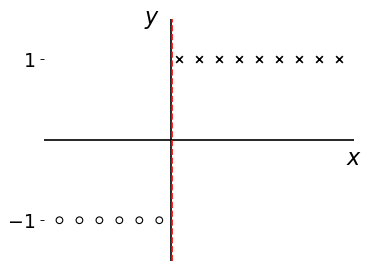
\includegraphics[width=0.9\textwidth]{img/neuron_1d_sign.png}
         }
         \caption{}
         \label{fig:neuron_1d_sign}
     \end{subfigure}
     \caption{Examples of different neuron responses to scalar input of two types: $\times$ and $\circ$. In \ref{fig:neuron_1d_sigmoid}: The neuron's response $y$ is continuous. In \ref{fig:neuron_1d_sign} the neuron repsonse is $+1$ for positive input and $-1$ otherwise. The red lines act as a decision boundary.}
	 \label{fig:neuron_1d}
\end{figure}

\end{frame}

\begin{frame}

\begin{figure}[ht]
     \centering
	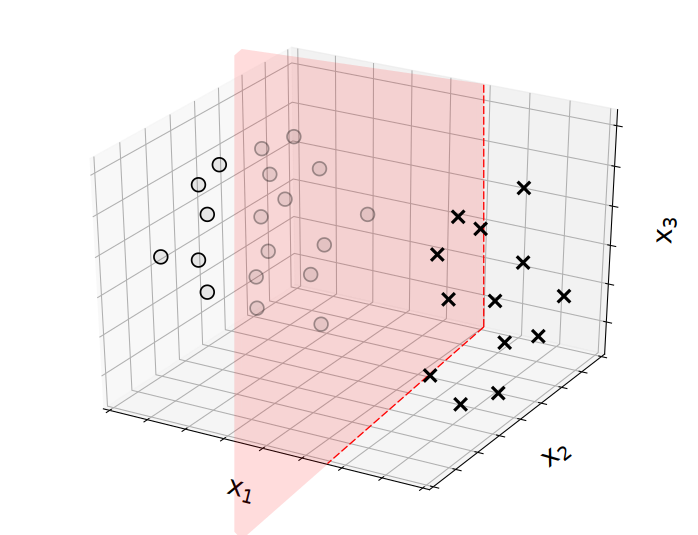
\includegraphics[width=0.4\textwidth]{img/neuron_3d_grid}
	\caption{Examples of a neuron's response to 3D input of types $\times$ and $\circ$. Inputs of different types fall on opposite sides of a plane. The red plane acts as a decision boundary}
	\label{fig:neuron_3d_grid} 
\end{figure}
\end{frame}


\subsection{Components of the connectionist neuron}
    
\begin{frame}
    
    \begin{figure}[h]
        \centering
        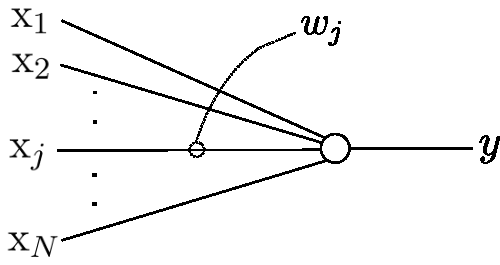
\includegraphics[height=2.5cm]{img/linearNeuron_y.pdf}
        \caption{The input-output relationship for a connectionist neuron. $w_{j}$ describes the connection from the $j$-th input.}
        \label{fig:neuron_diagram}
    \end{figure}
    
    \figref{fig:neuron_diagram} is a diagram of a connectionist neuron. Given an input vector $\vec x \in \R^{N}$ with components $x_{j}$,
    the connectionist neuron is composed of the following elements:

    \begin{enumerate}[(a)]
        \item weights $\vec w \in \R^{N}$: The weights represent the strength of the connections between the neuron and each component of the input it receives.\\
        
        \item A linear filter: Summation of the weighted inputs (e.g. scalar product: $\vec w^{\top} \vec x = \sum_{j} w_{j} x_{j}$).
        
        \item A bias value $\theta \in \R$ also known as the threshold of the neuron.\\
        

        
        \item An activation function or transfer function $f: \R \mapsto \R$. \\
        
        $f(\cdot)$ controls the range of the neuron's response. It can have the effect of squashing the response to a specific range of values or a specific set of values and preventing other value ranges.
        \item The scalar output of the neuron: $y$.
    \end{enumerate}
    
    \begin{figure}[h]
        \centering
        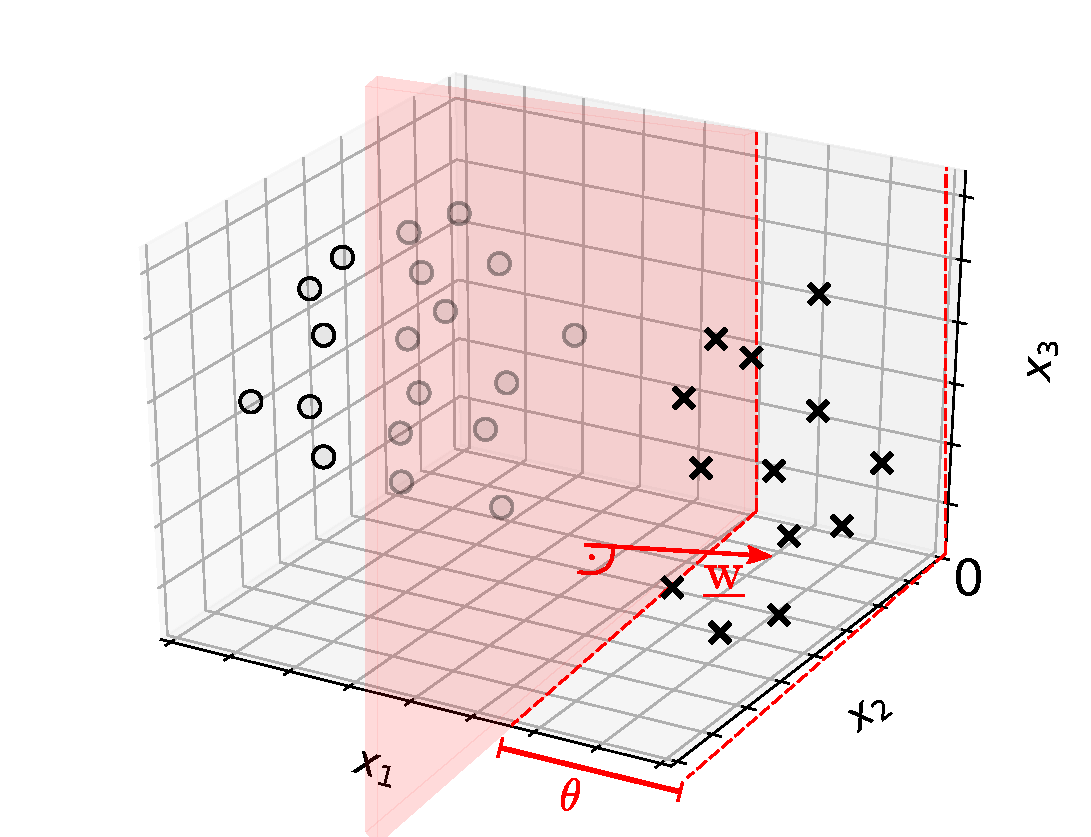
\includegraphics[height=6cm]{img/neuron_3d_grid_hyperplane.pdf}
        \caption{The hyperplane $\color{red}H = \set{\vec x : \vec w^{\top} \vec x = \theta}$ that divides the response of the neuron. In the context of classification it is referred to as the decision boundary.}
        \label{fig:neuron_3d_grid_hyperplane}
    \end{figure}
    
    The input-output relationship is described by a linear filter with a static non-linearity $f(\cdot)$:

    \begin{equation}
        \label{eq:linearNeuron}
        y = f \Big(\; \underbrace{\sum_{j=1}^{N} {w}_{j} 
            {x}_j - \theta}_{=:h} \; \Big)
            = f \big(\;  \vec{w}^{\top}
            \vec{x}- \theta \; \big)
            = f(\,h\,)
    \end{equation}
    
	\[ \begin{array}{ll} 
		\vec{x}: & \text{input vector with components } \mathrm{x}_j \\
		y: & \text{scalar output of the neuron } \\
		\vec{w}: & \text{weight vector of the neuron with components }
			\mathrm{w}_{j}\\
		\theta: & \text{threshold of the neuron} \\
		h: & \text{total input of the neuron. } h \propto \frac{\vec w^\top \vec x}{\;||\vec w||_2} \text{ component of $\vec x$ in the direction of $\vec w$}\\
		f(\cdot): & \text{transfer function}
	\end{array} \]
    
\end{frame}

\begin{frame}

\question{What roles do the weights and bias play?}

\pause
{}
\mode<article>{
\begin{itemize}
\item[-] $\vec w$ is effecively the normal vector of the hyperplane. Therefore, the weights represent the orientation of the hyperplane (see. \figref{fig:neuron_3d_grid_hyperplane}).
\item[-] $\theta$ represents the shift of the hyperplane (see. \figref{fig:neuron_3d_grid_hyperplane}). It is the absolute position of the hyperplane fron the origin along $\vec w$. For any point $\widetilde{\vec x} \in H$ (i.e. points on the plane): 
$\frac{\vec w^\top \widetilde{\vec x}}{\,||\vec w||_2} = \frac{\theta}{\,||\vec w||_2}$
\end{itemize}
}

\mode<presentation>{
    \begin{figure}
        \centering
        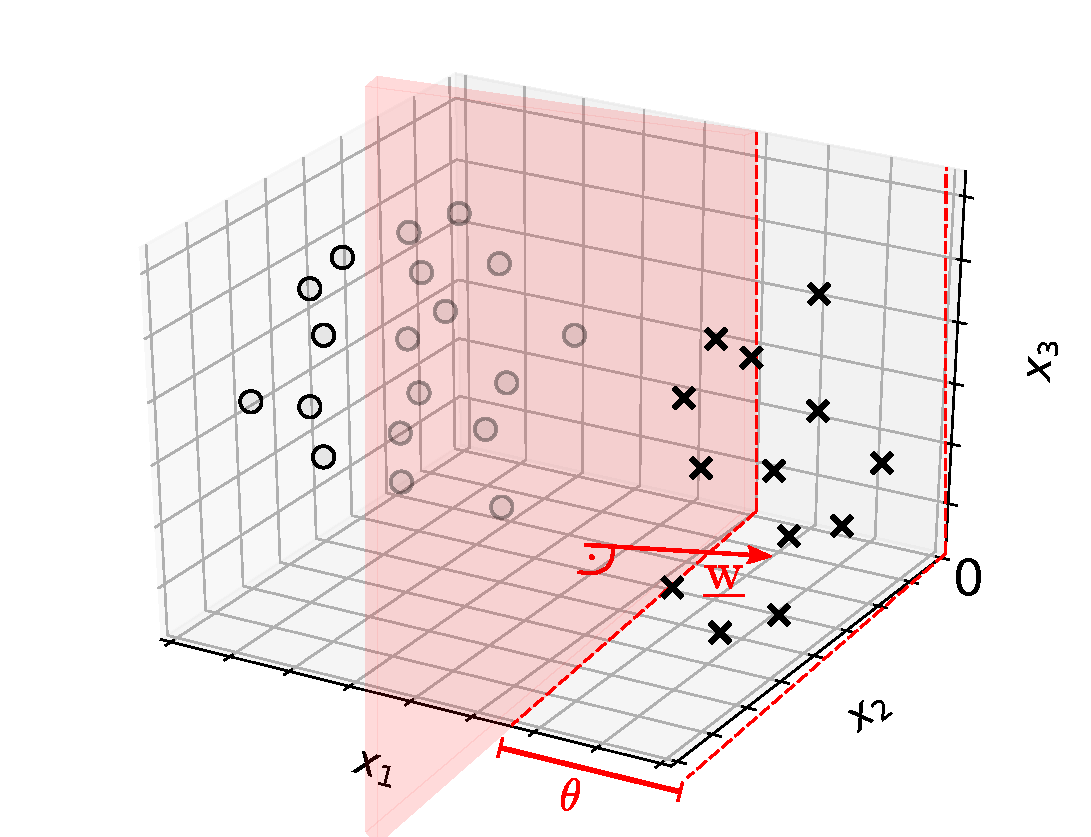
\includegraphics[height=6cm]{img/neuron_3d_grid_hyperplane.pdf}
        \caption{The hyperplane $\color{red}H = \{\vec x : \vec w^{\top} \vec x = \theta \}$ that divides the response of the neuron.}
    \end{figure}
}
\end{frame}

\subsection{Linear vs. non-linear transfer functions}

\begin{frame}


\question{What are the advantages of using a non-linear transfer function instead of a linear one?}

\begin{figure}[ht]
     \centering
     \savebox{\imagebox}{
	 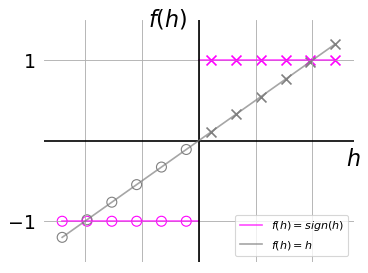
\includegraphics[width=0.3\textwidth]{img/neuron_1d_sign_and_linear}}%
     \begin{subfigure}[t]{0.35\textwidth}
         \centering
         \usebox{\imagebox}% Place largest image
         \caption{\footnotesize Linear vs. non-linear activation}
         \label{fig:linear_sign}
     \end{subfigure}
     \hspace{2mm}
     \begin{subfigure}[t]{0.35\textwidth}
         \centering
         \raisebox{\dimexpr.5\ht\imagebox-.5\height}{% Raise smaller image into place
         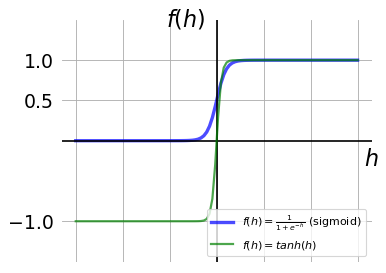
\includegraphics[width=0.9\textwidth]{img/neuron_1d_sigm_tanh}
         }
         \caption{\footnotesize logistic sigmoidal $\scriptstyle f(h)=\frac{1}{1+e^{-h}}$ vs. tanh}
         \label{fig:sigmoid_tanh}
     \end{subfigure}
     \mode<article>{
     \caption{Comparing linear with non-linear activation functions and differentiable alternatives to the sign function.}
     }
	 \label{fig:transfer_linear_nonlinear}
\end{figure}

\pause
- Advantages:
\begin{enumerate}
\item binary classification, either $f(h) \in \{0,1\}$ or $f(h) \in \{-1,1\}$
\item interpret $f(h)$ as a probability. The logistic sigmoidal where $f(h) = \frac{1}{1+exp(-h)}$ yields values in the range of (0,1). The logistic sigmoidal can also be obtained by shifting and scaling the tanh function (see \sectionref{sec:tanh_to_sigmoid}.
\item a multilayer perceptron with only linear transfer functions can be reduced to single layer. The hidden layers become redundant \footnote{Recent literature reveals interesting insights in what kind of representations are found across the layers of linear networks. For more information see Saxe, A. M., McClelland, J. L., \& Ganguli, S. (2019). A mathematical theory of semantic development in deep neural networks. Proceedings of the National Academy of Sciences, 116(23), 11537-11546.}:\\

     \begin{tabular}{c c c }
     		\raisebox{-9mm}{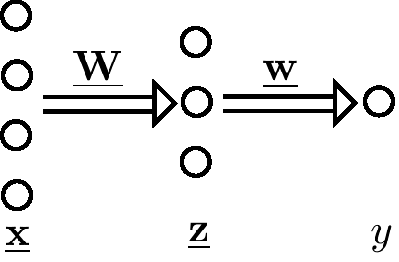
\includegraphics[height=2.25cm]{img/section1_fig16.pdf}}
     	& 
     		\begin{minipage}{10mm}
     			\vspace{10mm}
     		\end{minipage} 
     	& 
     		\parbox{4cm}{
		    \begin{eqnarray*}
		      y & = & \vec{w}^\top \vec{z}  
		      \quad = \quad \vec{w}^\top \vec{W} \, \vec{x} \\
		      & = & (\underbrace{\vec{W}^\top \vec{w}}_{=: \widehat{\vec{w}}})^\top \vec{x}
		      \quad = \quad \widehat{\vec{w}}^\top \vec{x}\\ 
		      & \corresponds & \text{connectionist neuron}
		    \end{eqnarray*}}
	\end{tabular}
\end{enumerate}


\end{frame}

\begin{frame}

\question{How does the logistic sigmoidal function relate to the tanh function?}

\mode<presentation>{
    \begin{figure}
        \centering
        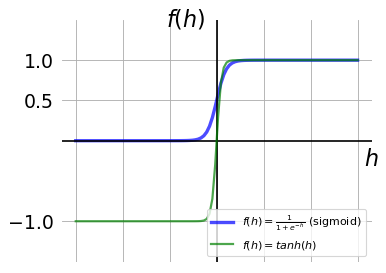
\includegraphics[height=6cm]{img/neuron_1d_sigm_tanh}
    \end{figure}
}

\mode<article>{

We observe in \figref{fig:sigmoid_tanh} that the logistic sigmoidal function (sigmoid) function is a shifted and scaled variant of the tanh function.
}

From this follows:
	\begin{align}
	f_{{\text{sigmoid}}}(h) 
    & = \frac{1}{1 + e^{-h}} \\
	& = \frac{e^{\frac{h}{2}}}{e^{\frac{h}{2}} + e^{-\frac{h}{2}}} \\
	& = \frac{1}{2} \Big(
		\underbrace{\frac{e^{\frac{h}{2}} - e^{-\frac{h}{2}}}{
			e^{\frac{h}{2}} + e^{-\frac{h}{2}}}}_{
				= \tanh \frac{h}{2}}
		+ \underbrace{\frac{e^{\frac{h}{2}} + e^{-\frac{h}{2}}}{
				e^{\frac{h}{2}} + e^{-\frac{h}{2}}}}_{= 1}
		\Big) \\
	& = \frac{1}{2} \left( \tanh \frac{h}{2} + 1 \right)
	\end{align}

    
\end{frame}

\subsection{Shortcut notation for weights and bias}

\begin{frame}

\mode<article>{
The bias is effectively a connection between the neuron and an input that is always on. 
We can absorb the bias into the weight vector by prepending it to $\vec w$ and prepending $\vec x$ with an element $x_0 = 1$:
}

    \begin{figure}[h]
        \centering
        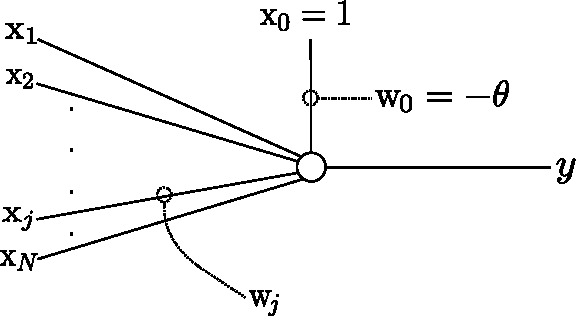
\includegraphics[height=3cm]{img/section1_fig6}
         \caption{Absorb bias into weight vector.}
         \label{fig:weight_with_bias}
    \end{figure}
 
\only<1>{
\mode<article>{   
The response of the neuron depicted in \figref{fig:weight_with_bias} can be computed by:
}

\begin{equation}
	y = f\big( \sum_{{\color{blue}j=0}}^{N} \mathrm{w}_j \mathrm{x}_j \big)
		= f( \vec{w}^\top \vec{x} )
	\label{eq:weight_with_bias}
\end{equation}

\mode<article>{

Note that the sum in \eqref{eq:weight_with_bias} now iterates from ${\color{blue}j=0}$ instead of $j=1$ as was done in \eqref{eq:linearNeuron} in order to include the bias element.
}

}

\only<2>{


	$\vec{w}$ will be used for $\rmat{ \mathrm{w}_1 \\ \vdots\;\,\\ \mathrm{w}_N}$ 
	as well as for $\rmat{ \mathrm{w}_0 \\ \mathrm{w}_1 \\ \vdots\;\, \\ \mathrm{w}_N}$. \\
	
	\rule{2cm}{0pt}
	
	Accordingly,
	$\vec{x}$ will be used for $\rmat{ \mathrm{x}_1 \\ \vdots\;\,\\ \mathrm{x}_N}$ 
	as well as for $\rmat{ \mathrm{x}_0 \\ \mathrm{x}_1 \\ \vdots\;\,\\ \mathrm{x}_N}$.
	
	Whether the bias is absorbed or not should become apparent from the context or explicitly from the limits of the sum.
}

\end{frame}

\mode*

\newpage

\mode<all>
\subsection{Limitations of Perceptrons}

\mode<article>{
Connectionist neurons, or perceptrons, are limited in the variety of functions they are able to fit. 
When dealing with classification problems, a perceptron can only find a linear separation between any two classes. Irrespective of the neuron's non-linear activation function, the perceptron is regarded as a \emph{linear classifier}. Whether something falls on one side of the decision boundary or the other, is entirely based on applying a linear filter (i.e. $\vec w^{\top} \vec x$). The non-linearity $f(h)$ merely controls the value range of the neuron's response ($\{0,1\}, (-1,+1)$, \ldots) which helps in interpreting the neuron's response.\\

If observations for two different classes are distributed such that one cannot draw a line to separate them, then the two classes
are not linearly separable. In this case, the perceptron will fail to find a suitable classification boundary between the two classes.
}

\begin{frame}\frametitle{Linear classifiers/linear decision boundaries}

Consider the following binary classification problems with $\vec x \in \R^2$.{}

\question{Can you find a line that separates the two classes for each case?}

\begin{figure}[h]
    \centering
	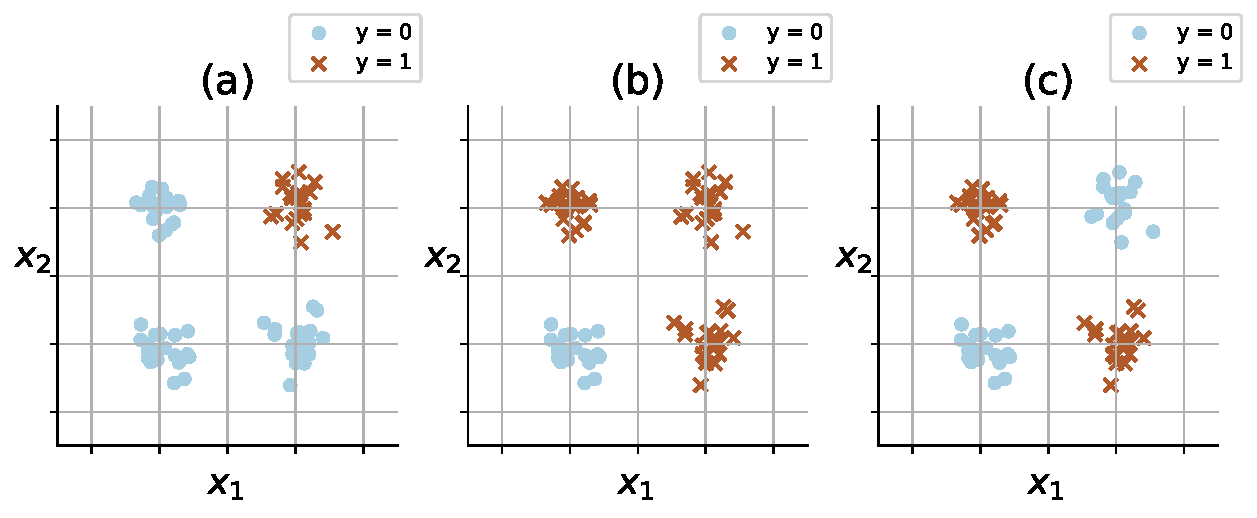
\includegraphics[width=0.8\textwidth]{img/and_or_xor_y}
	\mode<article>{
	\caption{(a) points are classified according to the AND function,
	(b) points are classified according to the OR function,
	(c) points are classified according to the XOR function.
	}
	}
	\label{fig:and_or_xor} 
\end{figure}

\mode<article>{
In \figureref{fig:and_or_xor}, particularly (a) and (b),
it is possible to draw a line that separates the classes. Therefore, the AND and OR functions are linearly separable.
A perceptron is capable of finding such a separating line. However, this does not apply to the third case, for the XOR function.
It is impossible to find a single line that will separate the classes.\\
The XOR function is not linearly separable.
}

\pause 

\question{Can we solve the XOR problem with multiple perceptrons? How?}\\

%\slidesonly{
%\begin{figure}[ht]
     %\centering
	%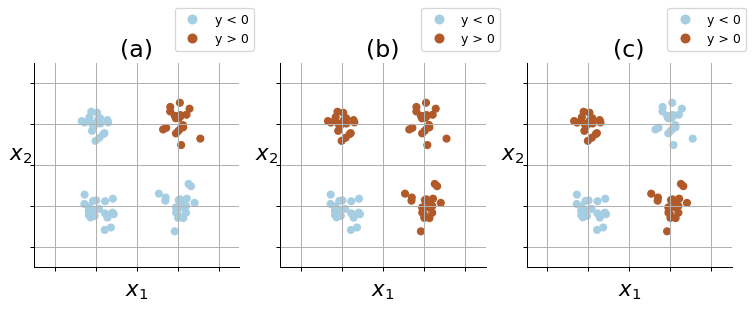
\includegraphics[trim=480 0 0 30, clip, width=0.4\textwidth]{img/and_or_xor_y.png}
	%\caption*{A single perceptron can not solve the XOR problem.}
	%\label{fig:xor} 
%\end{figure}
%}

\pause

\notesonly{
- Yes, think of it as a divide and conquer approach. We split the XOR problem into multiple sub-problems. 
A perceptron is used to solve each sub-problem.

If you're familiar with Boolean algebra, you might recognize the following expression for the XOR function:
}
\mode<presentation>{
\vspace{-10mm}
}

\begin{equation}
\label{eq:xor}
\mathrm{XOR}(x_1, x_2) = 
({\color{magenta}\,{x_1} \; \mathrm{AND} \; \overline{x}_2 \,})
 \;\; \mathrm{OR} \;\; 
({\color{green}\, \overline{x}_1 \; \mathrm{AND} \; x_2 \,})
\end{equation}

\end{frame}

\mode<article>{
For instance, the first perceptron ${\color{magenta}s^1_1}$ is tasked to separate the bottom-right cloud of points from the rest. 
A second perceptron ${\color{green}s^1_2}$ is used to separate the top-left cloud from the rest.
A third perceptron ${\color{blue}s^2_1}$ will then use the responses of both and respond to ``is \textbf{only one} of the two perceptrons \textbf{on}?''.

\figref{fig:build_xor} illustrates this approach. One need only recognize that each sub-problem is linearly separable.\\
}

\begin{frame}

\begin{figure}[ht]
    \centering
	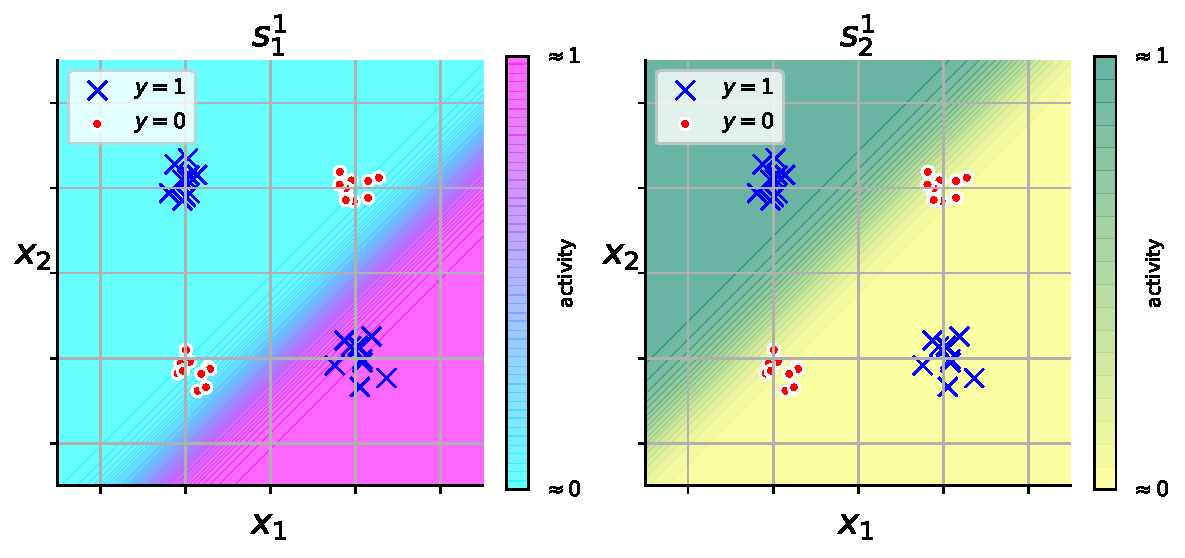
\includegraphics[width=0.75\textwidth]{img/build_xor_crf}
	\caption{Solving sub-problems of the XOR problem.}
	\label{fig:build_xor} 
\end{figure}

\end{frame}

\begin{frame}

\begin{figure}[ht]
    \centering
	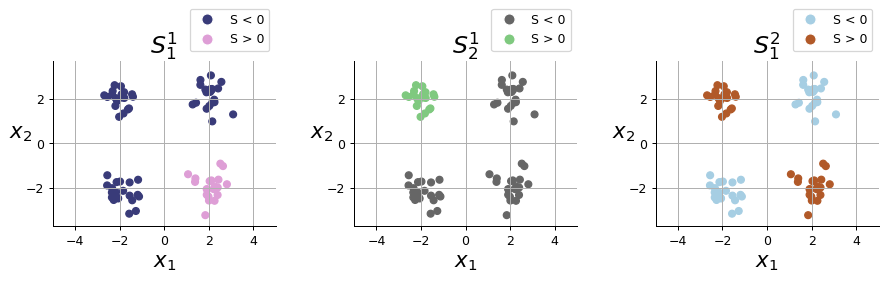
\includegraphics[width=0.75\textwidth]{img/build_xor}
	\caption{Solving sub-problems of the XOR problem.}
	\label{fig:build_xor} 
\end{figure}

\end{frame}


\mode<article>{
\figref{fig:xor_decisions} visualizes the response of the final neuron $s^2_1$ for different values of $x_1$ and $x_2$. The space is partitioned into one region in which the activity is $< 0.5$ and two disjoint regions (top-left \& bottom-right) in which the activity is $> 0.5$.
}

\begin{frame}
\begin{figure}[ht]
     \centering
     \savebox{\imagebox}{
     \mode<presentation>{
	 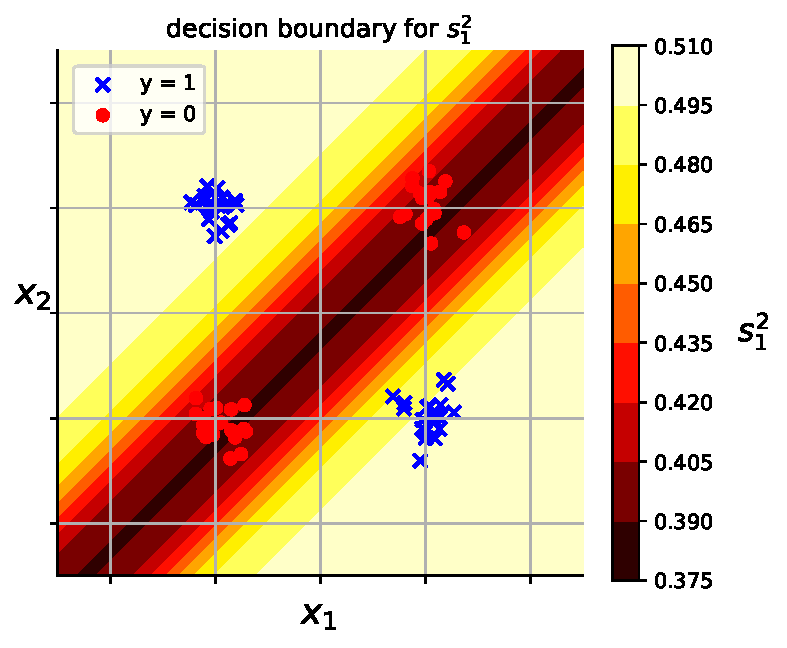
\includegraphics[width=0.4\textwidth]{img/xor_decision}
	 }
     \mode<article>{
	 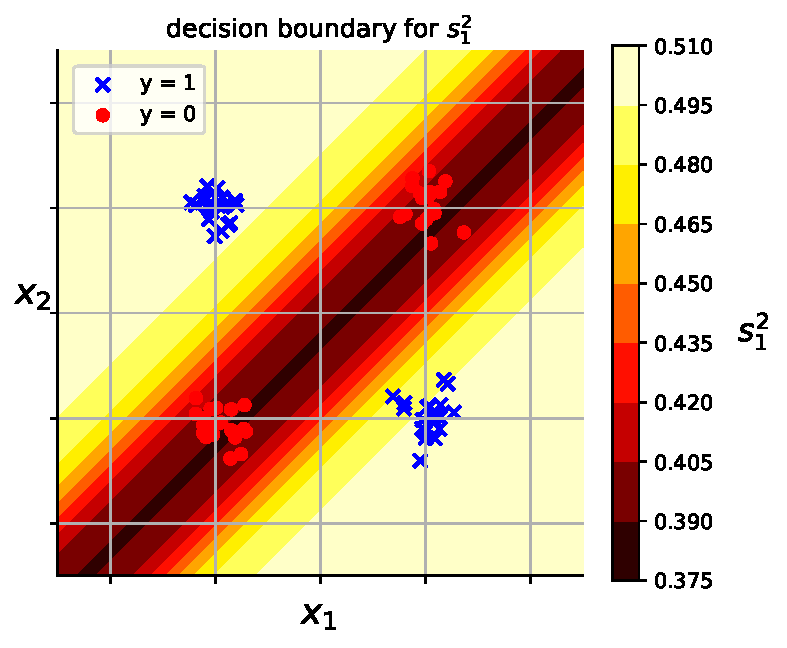
\includegraphics[width=0.35\textwidth]{img/xor_decision}
	 }
	 }%
     \begin{subfigure}[t]{0.35\textwidth}
         \centering
         \usebox{\imagebox}% Place largest image
         \caption{}
         \label{fig:xor_decisions}
     \end{subfigure}
     \slidesonly{
     \hspace{4mm}
     \begin{subfigure}[t]{0.45\textwidth}
     }
    \notesonly{
     \hspace{1mm}
     \begin{subfigure}[t]{0.38\textwidth}
     }
         \centering
         \raisebox{\dimexpr.5\ht\imagebox-.5\height}{% Raise smaller image into place
         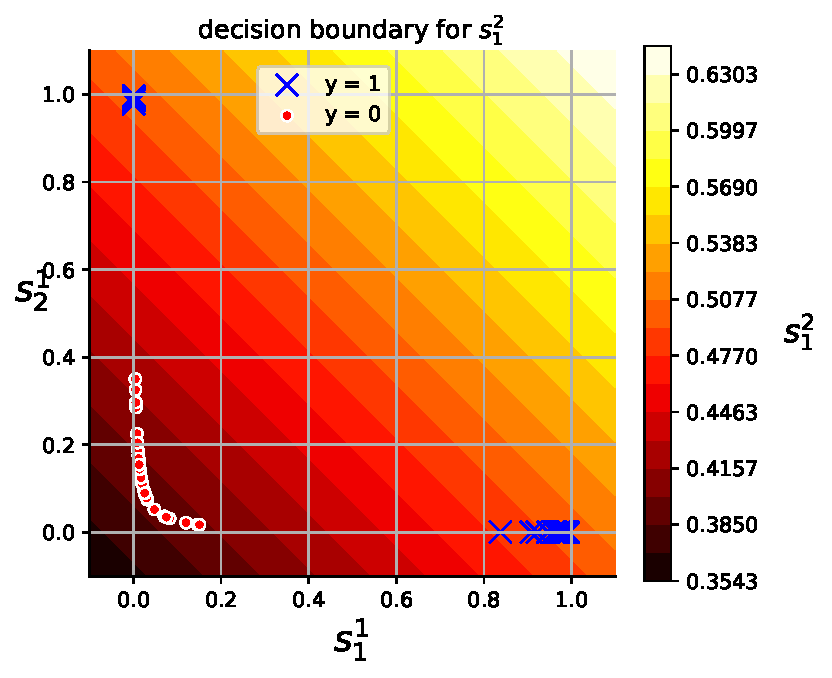
\includegraphics[width=0.9\textwidth]{img/xor_decision_s}
         }
         \caption{}
         \label{fig:xor_decisions_s}
     \end{subfigure}
	\caption{Identifying the decision boundaries.}
\end{figure}
\end{frame}

\newpage
\mode<article>{


What we are essentially describing is a Multilayered perceptron (MLP) with an architecture as illustrated in \figref{fig:xor_mlp_arch}. This MLP is made up of an output layer with a single output neuron ${\color{blue}s^2_1}$, and one hidden layer with two hidden neurons, ${\color{magenta}s^1_1}$ and ${\color{green}s^2_2}$ (the superscript denotes the layer index, the subscript denotes the neuron index within its layer). The terms ``neurons'' and ``nodes'' are treated as synonyms.
}
\begin{frame}

\begin{figure}[ht]
    \centering
	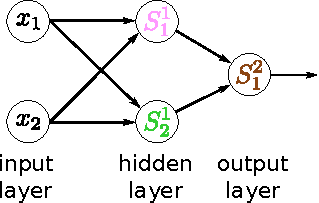
\includegraphics[width=0.4\textwidth]{img/xor_mlp_arch}
	\caption{simplified MLP architecture}
	\label{fig:xor_mlp_arch} 
\end{figure}



\end{frame}

\clearpage

\section{Feedforward MLP}
\subsection{Navigating through the indices}

\begin{frame}\frametitle{MLP}

\mode<article>{
The nodes in a feedforward neural network form a directed acyclic graph (DAG). There are no connections that feed back to a neuron in an earlier layer. A neuron can only be connected to another neuron that lies in a deeper layer in the network. We will eventually cover neural architectures that allow for feedback connections such as recurrent neural networks.
\figref{fig:mlp_arch} is an example MLP architecture (simplified by omitting bias nodes).
}

\begin{figure}[ht]
    \centering
	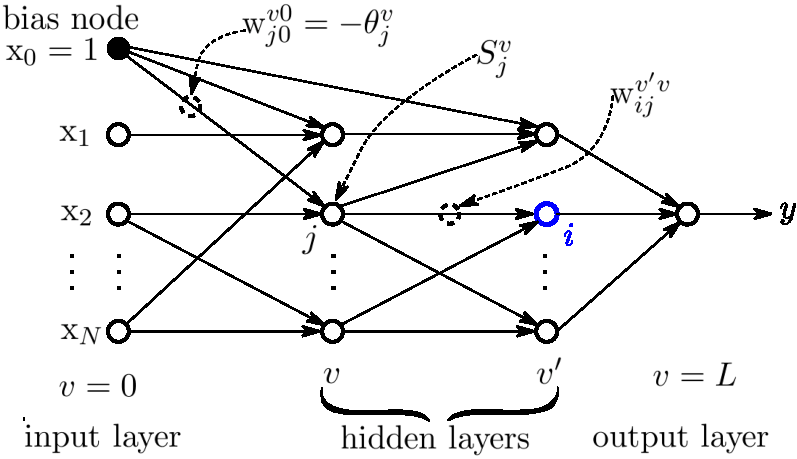
\includegraphics[width=0.7\textwidth]{img/section1_fig14}
	\caption{MLP architecture}
	\label{fig:mlp_arch} 
\end{figure}

\mode<article>{
Each node in the network is a connectionist neuron. This implies that every individual neuron extracts some feature from the ``input'' it receives.
The ``input'' to a neuron can come from the observed data $\vec x$ or it could be the response of another neuron from an earlier layer in the network.
This also implies that \emph{for every neuron} their exists a hyperplane which is represented by some weights $\vec w$ and a bias $\theta$.

$s^v_j$ denotes the \emph{activity} of the neuron $j$-th in layer $v$, while $s^{v'}_i$ denotes the \emph{activity} of the neuron $i$-th in layer $v'$.
$h^v_j$ and $h^{v'}_i$ denotes the \emph{total input} for neuron $(v,j)$ and neuron $(v',i)$, respectively.
The activity $s^{v'}_i$ is obtained by applying a transfer function $f^{v'}_i(\cdot)$ to the total input $h^{v'}_i$ of neuron $(v',i)$:
}

\begin{equation}
s^{v'}_i = f^{v'}_i(h^{v'}_i)
\end{equation}

\mode<article>{
where common choices for $f^v_j(\cdot)$, depending on the layer, can be:
\begin{itemize}
\item the identity function: $f^v_j(h) := h$. Often for the input layer, i.e. $s^0_j = f^0_j(h^0_j) = f^0_j(x_j) = x_j$
\item logistic sigmoidal or $\tanh(h)$. Common for hidden neurons and output neurons (for classification tasks).
\end{itemize}

$v$ is a literal that is used to denote a specific layer in the network.\\
$v=0$ describes the \emph{input layer} which holds the observations $\vec x$.\\
$v=L$ describes the \emph{output layer} of the MLP. All the layers in between, if any, are referred to as \emph{hidden layers}. For example, the scalar output of an MLP can be referred to using:


\begin{equation}
y(\vec x;\vec w) = f^L_1(h^L_1)
\end{equation}

$v'$, $v''$ are used to describe layers relative to the current layer $v$. $v'=v+1$ and $v''=v'+1=v+2$ is a very common but this depends on how exactly any two nodes are connected. Therefore, talking about layers $v$, $v'$ and $v''$ needs to be put into the context of the connections between neurons. To elaborate:

$w_{ij}^{v'v}$ measures the strength of the connection \underline{from} $(v,j)$ \underline{to} $(v',i)$. Seeing $v'v$ in the superscript of the weight tells us that the two neurons are directly connected (1 hop).

$w_{j0}^{v0}$ measures the bias $-\theta_{j0}^{v0}$ for neuron $(v,j)$. 

}

\end{frame}

\definecolor{darkgreen}{rgb}{0,0.6,0}
\begin{frame}
\only<1>{\frametitle{MLP}
}
\only<2>{\frametitle{MLP with \textbf{fully connected} layers}
}

\mode<presentation>{
\begin{figure}[ht]
     \centering
     \savebox{\imagebox}{
     \only<1>{
	 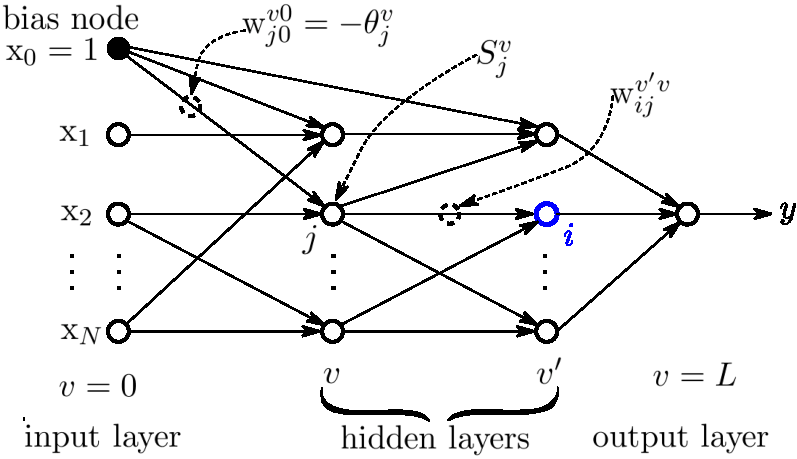
\includegraphics[width=0.4\textwidth]{img/section1_fig14}%
	 }
     \only<2->{
	 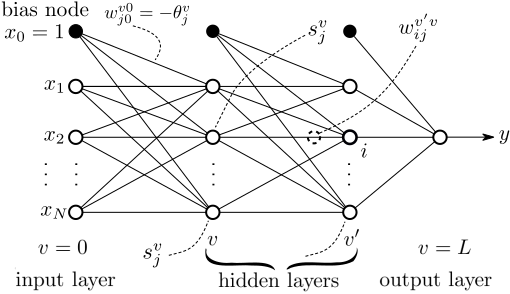
\includegraphics[width=0.4\textwidth]{img/section1_fig14_fc}%
	 }}%
     \begin{subfigure}[t]{0.5\textwidth}
         \centering
         \usebox{\imagebox}% Place largest image
     \end{subfigure}
     \hspace{10mm}
     \begin{subfigure}[t]{0.3\textwidth}
         \centering
         \raisebox{\dimexpr.5\ht\imagebox-.5\height}{% Raise smaller image into place
         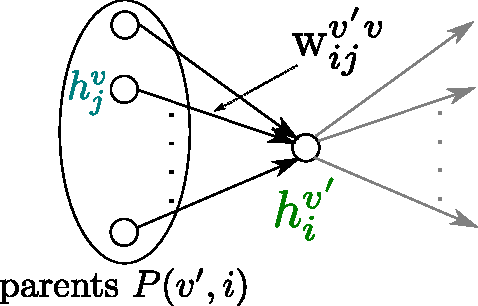
\includegraphics[width=0.9\textwidth]{img/section1_fig20_mini_vdi}
         }
     \end{subfigure}
\end{figure}
}

\mode<article>{

\begin{figure}
    \centering
	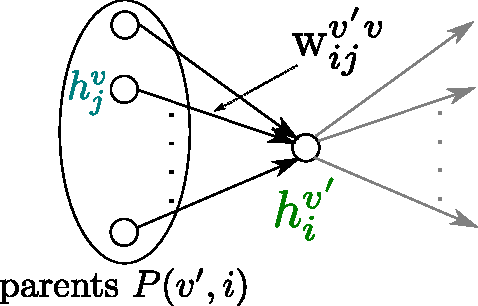
\includegraphics[width=0.33\textwidth]{img/section1_fig20_mini_vdi}
	\caption{Computing the total input for neuron $(v',i)$}
	\label{eq:compute_vdi}
\end{figure}
}

\mode<article>{
To formulate how neuron $(v', i)$ processes its input requires identifying the set of parent nodes $P(v', i)$ of neuron $(v',i)$. The weighted sum of the parent activations yields the total input ${\color{darkgreen}h^{v'}_i}$:
}
   
\only<-2>{
\begin{equation}
		{\color{darkgreen}h_i^{v'}} 
		:= 
		\kern-2ex
		\sum_{(\mu,k) \in P(v',\,i)}
		\kern-2ex
		w_{ik}^{v'\mu}\; 
		f_k^\mu\big( {\color{teal} h_k^\mu} \big)   
		\label{eq:total_input_vdi_pre},
\end{equation}
}

\mode<article>{
We now assume an architecture with \emph{fully connected layers}. This implies that every node in layer $v$ is connected to all nodes in the subsequent layer $v'$ (except for the bias node in $v'$ because it has no parents). This type of connectivity allows us to simplify the notation as it implies that the set of parents $P(v',\,i)$ is essentially a vector of all activations in layer $v$:
}

\only<2>{
\slidesonly{
Full connectivity implies
}
\begin{equation}
P(v',i) := (
\underbrace{
s^v_0}_{\substack{=1\\ \text{(bias)}}
}
, s^v_1, \ldots, s^v_j, \ldots, s^v_{N_v})^\top,
\end{equation}

where $N_v$ is the number of hidden nodes in layer $v$. 

\notesonly{From this follows:}
}

\only<3>{

\begin{align}
		{\color{darkgreen}h_i^{v'}} 
		:=& 
		\kern-2ex
		\sum_{(\mu,k) \in P(v',\,i)}
		\kern-2ex
		w_{ik}^{v'\mu}\; 
		f_k^\mu\big( {\color{teal} h_k^\mu} \big) \\
		{\color{darkgreen}h_i^{v'}} \;
		\stackrel{\mathclap{
\substack{\text{\tiny fully}\\\text{\tiny conn.}}}
}{=}& 
		\kern1.5ex
		\sum_{j=0}^{N_v}
		w_{ij}^{v'v}\; 
		f_j^v\big( {\color{teal} h_j^v} \big)\\
		=& 
		\kern1.5ex
		{\vec w_{i}^{v'v}}^\top
		\kern-1ex
		\cdot  
		\vec f^v\big( {\color{teal} \vec h^v} \big)\\
		=& 
		\kern1.5ex
		{\vec w_{i}^{v'v}}^\top
		\kern-1ex
		\cdot
		\vec s^v\\
\end{align}

\slidesonly{\vspace{-5mm}}
here $\vec w_{i}^{v'v} := \big(
\underbrace{
w_{i0}^{v'v}}_{\text{bias}}
, w_{i1}^{v'v}, \ldots,w_{iN_v}^{v'v}\big)^\top \in \R^{N_v+1}$
}

\only<4>{
\notesonly{
Consequently, to compute} the total input for all $N_{v'}$ neurons in the layer $v$\notesonly{ we introduce the weight matrix 
$\vec W^{v'v} := \big({\vec w_1^{v'v}}^\top, {\vec w_2^{v'v}}^\top, \ldots, {\vec w_{N_{v'}}^{v'v}}^\top\big)$:}
\begin{equation}
\vec W^{v'v} = 
\left(
\begin{array}{cccccc}
\Big| & \Big| & & \Big| & & \Big| \\[3mm]
\vec w_{1}^{v'v} & \vec w_{2}^{v'v} & \cdots & \vec w_{i}^{v'v} & \cdots & \vec w_{N_{v'}}^{v'v}\\[2mm]
\Big| & \Big| & & \Big| & & \Big|
\end{array}
\right) \in \R^{(N_v+1) \times N_{v'}}
\end{equation}

Therefore,

\begin{equation}
		{\color{darkgreen} \vec h^{v'}} 
		=
		{\vec W^{v'v}}^\top
		\kern-1ex
		\cdot
		\vec f^v\big( {\color{teal} \vec h^v} \big)
		=
		\kern1.5ex
		{\vec W^{v'v}}^\top
		\kern-1ex
		\cdot
		\vec s^v
\end{equation}
}

\end{frame}

\mode*

\end{rightcolumn}
\end{paracol}

\end{document}
